\begin{solutionfigure}
\centering
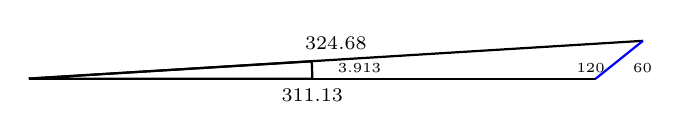
\begin{tikzpicture}[scale=1.2]
    % Basislinie (horizontale Achse)
    \draw[black, thick] (0,0) -- (6,0) node[midway, below] {\scriptsize \SI{311.13}{\volt}};


    % Oberer Vektor (mit Winkel)
    \draw[black, thick] (0,0) -- (6.5,0.4) node[midway, above] {\scriptsize \SI{324.68}{\volt}};
    \def\drawArc#1#2#3{
    \draw[thick] (#1:0) -- (#1:#3) arc (#1:#2:#3) -- cycle;
    }
        % Beispiel: Kreissegment von 0 bis 60 Grad mit Radius 0.6
    \drawArc{0}{3.5}{3}{color=blue!70!black};
    \draw[blue,thick] (6.5,0.4) -- (6,0);

    \node at (6.2,0.11) [left] {\tiny \SI{120}{\degree}};
    \node at (6.7,0.11) [left] {\tiny \SI{60}{\degree}};
    \node at (3.5,0.11) {\tiny \SI{3.913}{\degree}};

  
\end{tikzpicture}
\caption{Illustration for determining the angle using the sine theorem.}
\label{fig:Illustration for determining the angle using the sine theorem}
\end{solutionfigure}
